% Unofficial University of Cambridge Poster Template
% https://github.com/andiac/gemini-cam
% a fork of https://github.com/anishathalye/gemini
% also refer to https://github.com/k4rtik/uchicago-poster

\documentclass[final]{beamer}

% ====================
% Packages
% ====================

\usepackage[T1]{fontenc}
\usepackage{lmodern}
\usepackage[orientation=portrait,size=a1]{beamerposter}
\usetheme{gemini}
\usecolortheme{nott}
\usepackage{graphicx}
\usepackage{booktabs}
\usepackage{tikz}
\usepackage{pgfplots}
\pgfplotsset{compat=1.14}
\usepackage{anyfontsize}
\usepackage{kotex}
\usepackage{amsmath}
\usepackage{mathtools}
\usepackage{amssymb}
\usepackage[labelformat=empty]{caption}
\usepackage{subcaption}
\usepackage{algpseudocode}


\captionsetup[subfigure]{labelformat=empty}

% ====================
% Lengths
% ====================

% If you have N columns, choose \sepwidth and \colwidth such that
% (N+1)*\sepwidth + N*\colwidth = \paperwidth
\newlength{\sepwidth}
\newlength{\colwidth}
% \setlength{\sepwidth}{0.025\paperwidth}
% \setlength{\colwidth}{0.45\paperwidth}

% \newcommand{\separatorcolumn}{\begin{column}{\sepwidth}\end{column}}


% ====================
% Title
% ====================

%\title{Arc Indices of Theta-Curves and Handcuff Graphs}
\title{Minimal Grid Diagrams of \\ Theta-Curves and Handcuff Graphs Up to 7 Crossings}


\author{Cho, Eunchan \inst{1} \and  Shin, Jeongwon \inst{1} \and  Seo, Boyeon \inst{1} \and  Choi, Minho \inst{1} \and Kim, Hun \inst{2} \and Jin, Gyo Taek \inst{3}}

\institute[shortinst]{\inst{1} Korea Science Academy of KAIST \samelineand \inst{2} Supervisor, Korea Science Academy of KAIST \samelineand \inst{3} Supervisor, asdf \samelineand}

% ====================
% Footer (optional)
% ====================

\footercontent{
  \begin{center}
    \begin{minipage}[c]{\linewidth}
      \centering
      \quad 
\includegraphics[height=2cm]{../Midterm_Poster/logos/ksa_logo.jpg} \hfill
      \centering
      
\includegraphics[height=2cm]{../Midterm_Poster/logos/kaist_logo.png} \hfill
      \centering
      
\includegraphics[height=2cm]{../Midterm_Poster/logos/gwaguibu_logo.png} \quad
    \end{minipage}

    \vspace{0.3cm}

    Korea Science Academy of KAIST \quad
    \href{http://www.ksa.hs.kr}{ksa.hs.kr} \quad
  \end{center}
}


% ====================
% Logo (optional)
% ====================

% use this to include logos on the left and/or right side of the header:
% \logoright{
\includegraphics[height=2.5cm]{logos/utfpr-logo.png}}
% \logoleft{\hspace{20ex}
\includegraphics[height=3.5cm]{logos/ppgca-logo.png}}

% ====================
% Body
% ====================



\begin{document}

% Refer to https://github.com/k4rtik/uchicago-poster
% logo: https://www.cam.ac.uk/brand-resources/about-the-logo/logo-downloads
% \addtobeamertemplate{headline}{}
% {
%     \begin{tikzpicture}[remember picture,overlay]
%       \node [anchor=north west, inner sep=3cm] at ([xshift=-2.5cm,yshift=1.75cm]current page.north west)
%       {\includegraphics[height=7cm]{logos/unott-logo.eps}}; 
%     \end{tikzpicture}
% }

\begin{frame}[t]
% \begin{columns}[t]
% \separatorcolumn

% \begin{column}{\colwidth}
\begin{columns}[t]
  \column{0.33\textwidth}
  \begin{block}{Definitions}
    %\textbf{Knot} is an embedding of a circle in 3-dimensional Euclidean space.
    %In \textbf{Knot Theory}, people classify each knot using their \textbf{Knot Invariant}. \\
    \begin{itemize}
      \item \textbf{theta-curve} : a spatial knot on 3-sphere which has 2 vertices and 3 edges
      %In the projection of the theta-curve, the section where theta-curve meets itself is named \textbf{crossing}.
      %If the one theta-curve and other theta-curve's continuous transform of the graph is same, these curves are \textbf{equivalent}.
      \item \textbf{handcuff graph} : consists of two loops and an edge joining the loops
      \item \textbf{generalized Reidemeister move} : used to transform a projection of theta-curve
    \end{itemize}
    \begin{figure}
      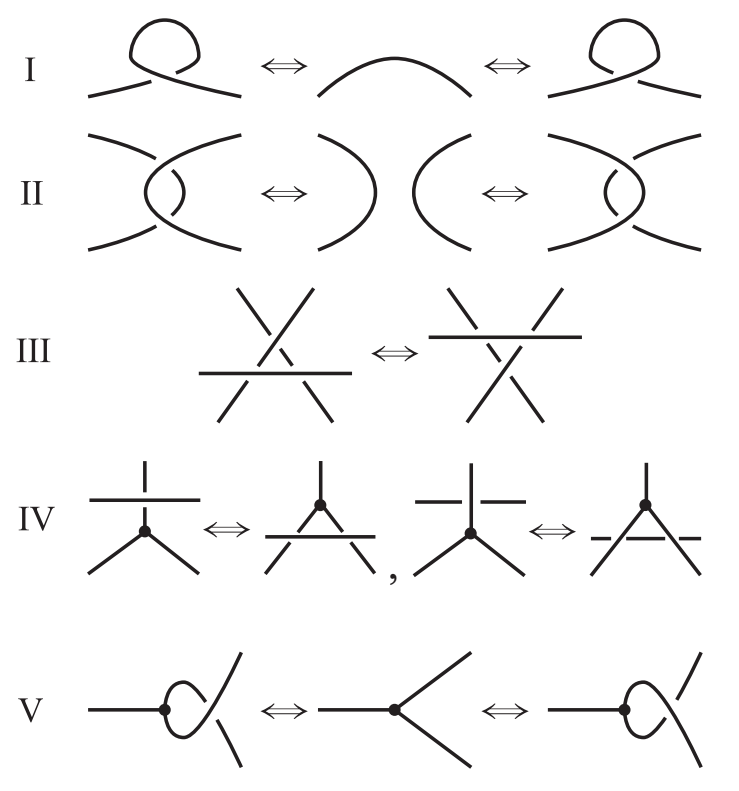
\includegraphics[width = 7.5cm]{figure/reidemeister.png}
      \caption{reidemeister moves for theta and hundcuff knots}
    \end{figure}
    
  \end{block}
    \column{0.33\textwidth}
  \begin{block}{Diagrams}

    \begin{Diagrams}
      \caption{An algorithm with caption}\label{alg:cap}
      \begin{itemize} 
        \item \textbf{grid diagram} : made of horizontal lines and vertical lines, and vertical lines are always on top of horizontal lines
        \item \textbf{Cromwell matrix} : matrix made of 0 and 1 - except 2 rows, each row and columns has exactly two 1s, and for 2 rows, there are exactly three 1s, if the 1s are connected by horizontal and vertical lines, it leads to the grid diagram
        \item \textbf{arc presentation} : can be expressed by grid diagram and vice versa \\ number of half planes are $\alpha$ on minimal arc presentation $\Rightarrow$ the size of corresponding grid diagram is $(\alpha - 1) \times \alpha$.\\
      \end{itemize} 
    \end{Diagrams}

  \end{block}
  \column{0.33\textwidth}
  \begin{block}{Classifying Theta-Curves and Handcuff Graphs by Determinant}
    $\mathbf{Definition.}$ The \textbf{THC-Cromwell matrix} is the matrix that satisfies the following conditions.
    \begin{enumerate}
      \item It is a $n\times(n+1)$ matrix with entries 0 and 1.
      \item It has only two `1's in every row and column, except for two rows. These two rows have three `1's.
    \end{enumerate}
    $\mathbf{Definition}$ Let any exception row(with three `1's) $i$ and its two outer `1's $j$, $k$.
    The \textbf{H-deletion Matrix} of THC-Cromwell matrix is $(n-1)\times(n-1)$ matrix which deleted row $i$ and column $j$, $k$.\\
    $\mathbf{Theorem.}$ The given THC-Cromwell matrix is theta-curve if and only if determinant of the H-deletion matrix is $\pm 1$.
    The given THC-Cromwell matrix is handcuff graph if and only if determinant of the H-deletion matrix is $0$ or $\pm 2$.\\
  \end{block}
\end{columns}

 \begin{alertblock}{Grid Diagram of the Theta-Curves and Handcuff Graphs Up to 7 Crossings}
  \hspace{1cm}
  \begin{columns}[t]
  \begin{column}{0.7\textwidth}
  \begin{alertblock}{Theta-Curves}
  \begin{figure}
    \begin{subfigure}{0.075\textwidth}
    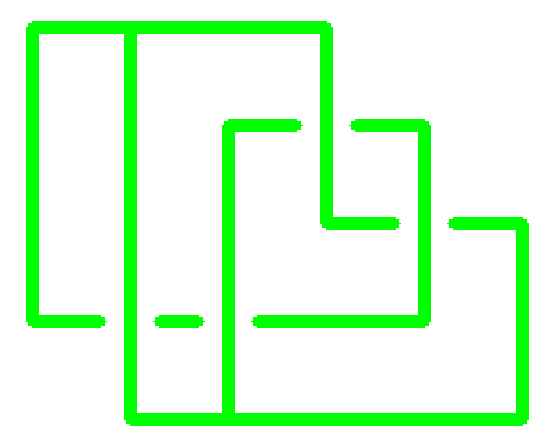
\includegraphics[width=2.5cm]{../Midterm_Poster/grid_diagram/theta_3_1.png}
    \caption{$3_1$} 
    \end{subfigure}
    \begin{subfigure}{0.075\textwidth}
    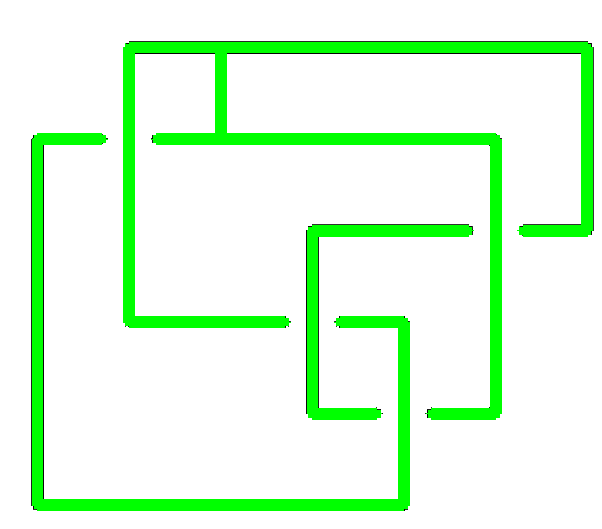
\includegraphics[width=2.5cm]{../Midterm_Poster/grid_diagram/theta_4_1.png}
    \caption{$4_1$} 
    \end{subfigure}
    \begin{subfigure}{0.075\textwidth}
    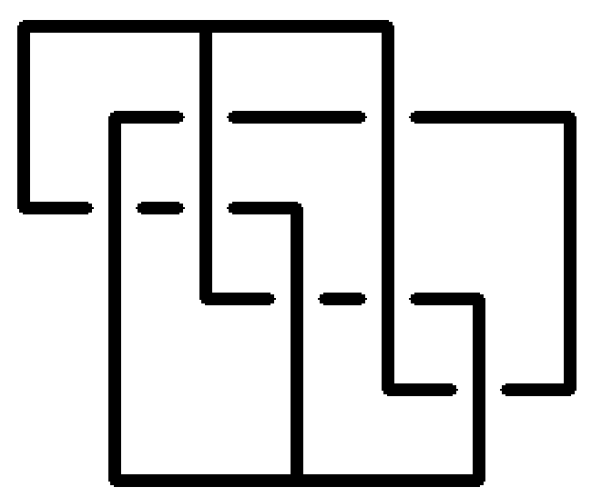
\includegraphics[width=2.5cm]{../Midterm_Poster/grid_diagram/theta_5_1.png}
    \caption{$5_1$}
    \end{subfigure}
    \begin{subfigure}{0.075\textwidth}
    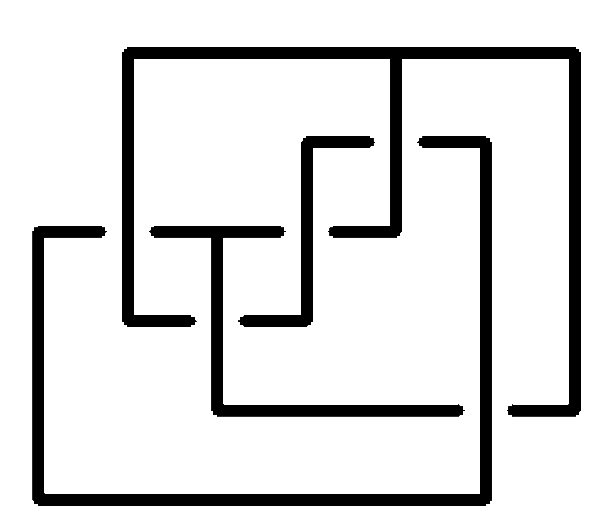
\includegraphics[width=2.5cm]{../Midterm_Poster/grid_diagram/theta_5_2.png}
    \caption{$5_2$} 
    \end{subfigure}
    \begin{subfigure}{0.075\textwidth}
    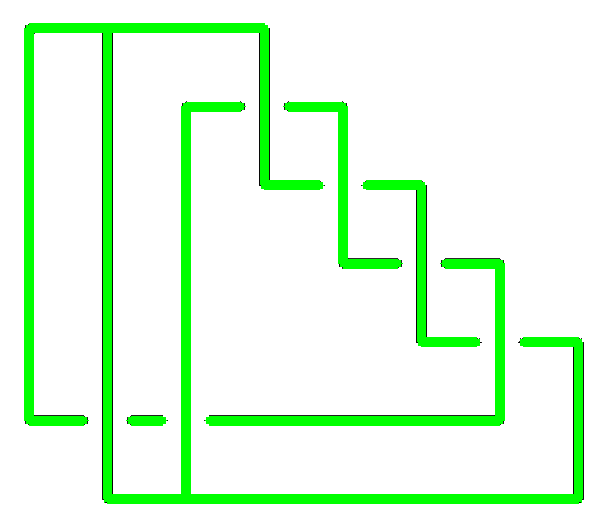
\includegraphics[width=2.5cm]{../Midterm_Poster/grid_diagram/theta_5_3.png}
    \caption{$5_3$}
    \end{subfigure}
    \begin{subfigure}{0.075\textwidth}
    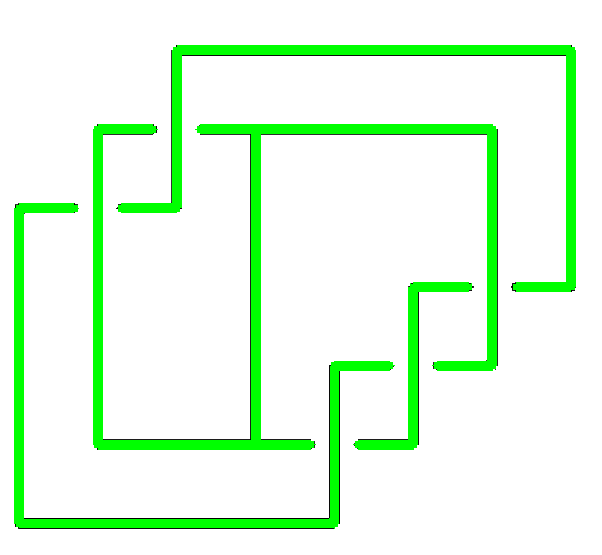
\includegraphics[width=2.5cm]{../Midterm_Poster/grid_diagram/theta_5_4.png}
    \caption{$5_4$} 
    \end{subfigure}
    \begin{subfigure}{0.075\textwidth}
    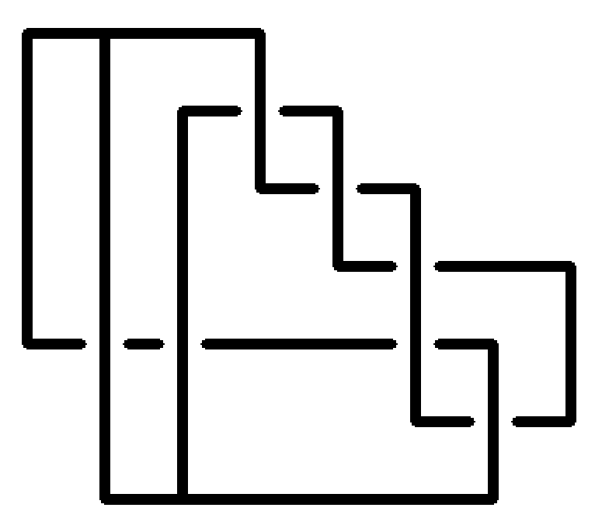
\includegraphics[width=2.5cm]{../Midterm_Poster/grid_diagram/theta_5_5.png}
    \caption{$5_5$} 
    \end{subfigure}
    \begin{subfigure}{0.075\textwidth}
    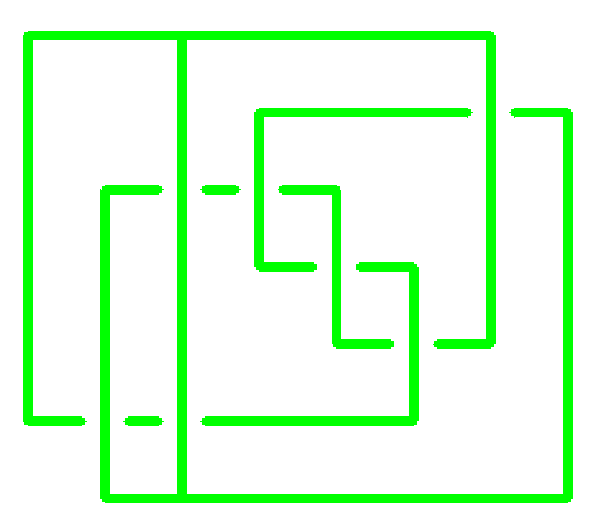
\includegraphics[width=2.5cm]{../Midterm_Poster/grid_diagram/theta_5_6.png}
    \caption{$5_6$} 
    \end{subfigure}
    \begin{subfigure}{0.075\textwidth}
    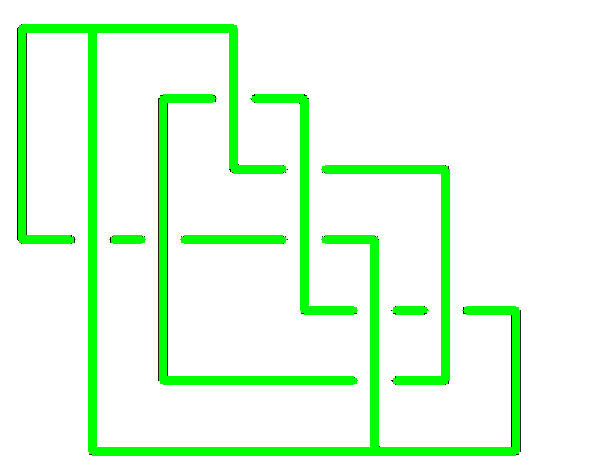
\includegraphics[width=2.5cm]{../Midterm_Poster/grid_diagram/theta_5_7.png}
    \caption{$5_7$} 
    \end{subfigure}
    \begin{subfigure}{0.075\textwidth}
    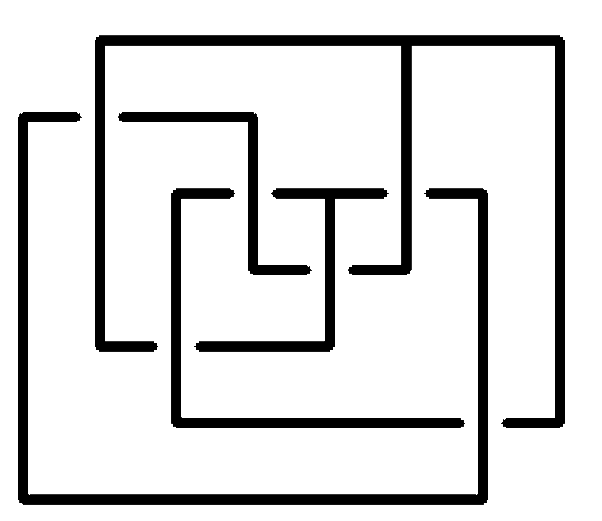
\includegraphics[width=2.5cm]{../Midterm_Poster/grid_diagram/theta_6_1.png}
    \caption{$6_1$} 
    \end{subfigure}
    \begin{subfigure}{0.075\textwidth}
    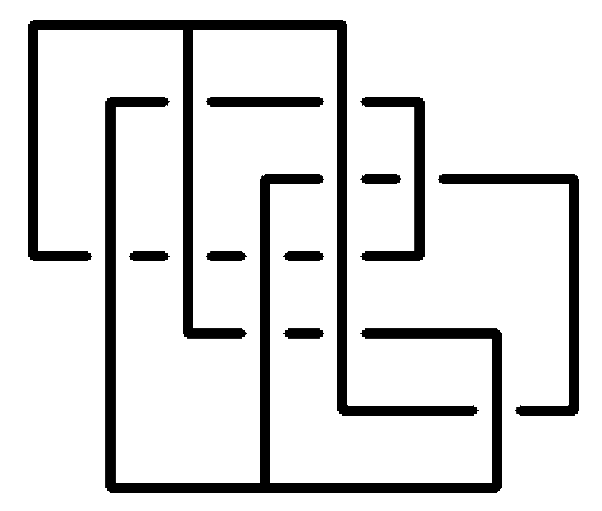
\includegraphics[width=2.5cm]{../Midterm_Poster/grid_diagram/theta_6_2.png}
    \caption{$6_2$} 
    \end{subfigure}
    \begin{subfigure}{0.075\textwidth}
    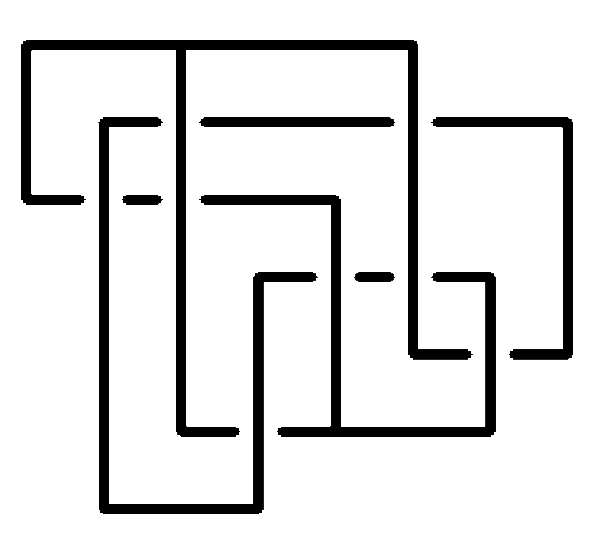
\includegraphics[width=2.5cm]{../Midterm_Poster/grid_diagram/theta_6_3.png}
    \caption{$6_3$} 
    \end{subfigure}
    \begin{subfigure}{0.075\textwidth}
    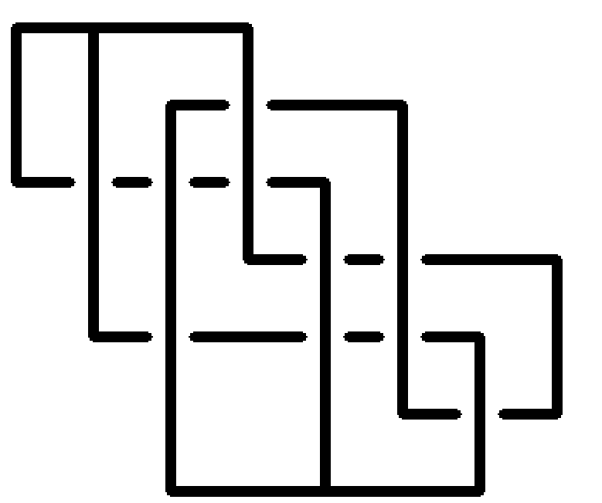
\includegraphics[width=2.5cm]{../Midterm_Poster/grid_diagram/theta_6_4.png}
    \caption{$6_4$} 
    \end{subfigure}
    \begin{subfigure}{0.075\textwidth}
    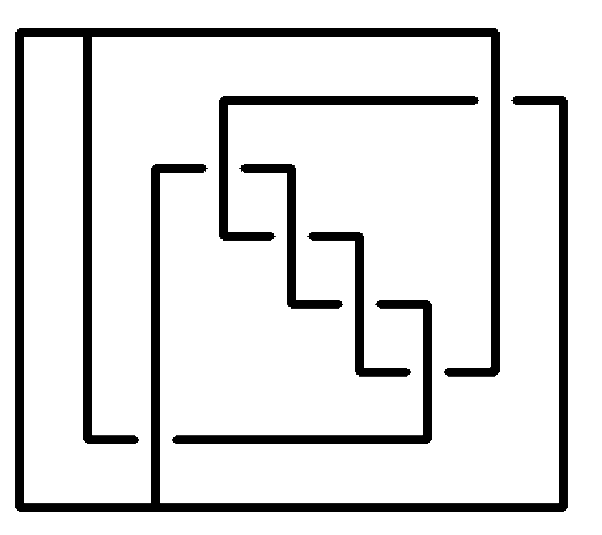
\includegraphics[width=2.5cm]{../Midterm_Poster/grid_diagram/theta_6_5.png}
    \caption{$6_5$} 
    \end{subfigure}
    \begin{subfigure}{0.075\textwidth}
    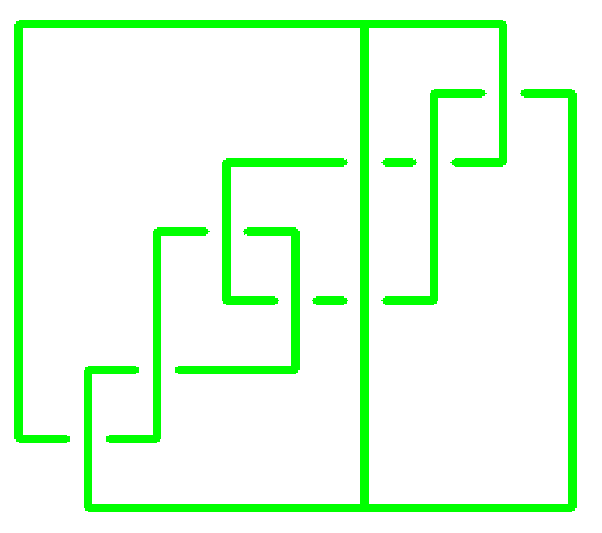
\includegraphics[width=2.5cm]{../Midterm_Poster/grid_diagram/theta_6_6.png}
    \caption{$6_6$} 
    \end{subfigure}
    \begin{subfigure}{0.075\textwidth}
    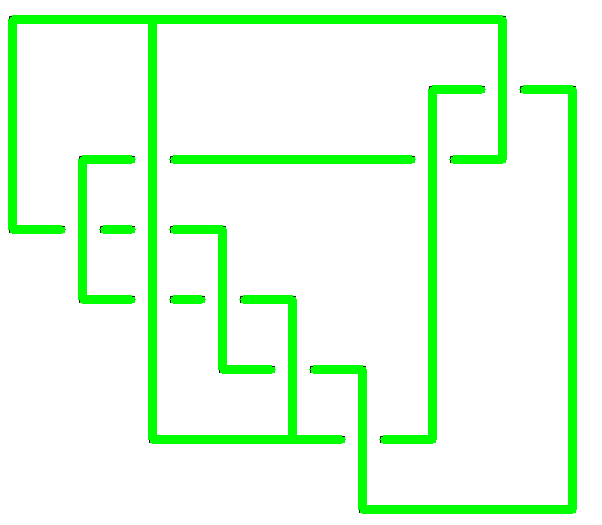
\includegraphics[width=2.5cm]{../Midterm_Poster/grid_diagram/theta_6_7.png}
    \caption{$6_7$} 
    \end{subfigure}
      \begin{subfigure}{0.075\textwidth}
    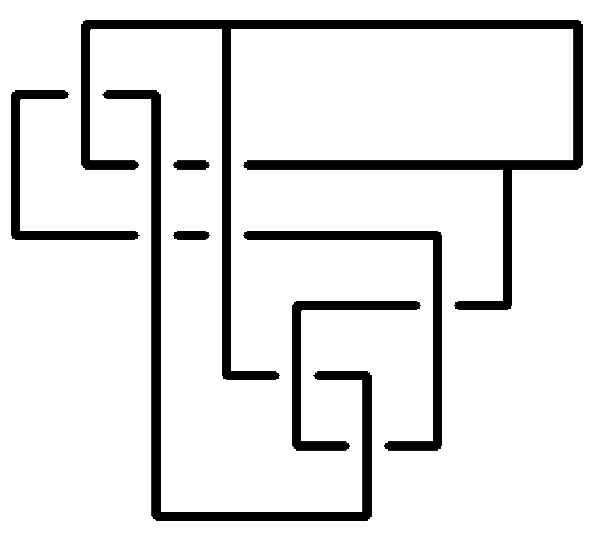
\includegraphics[width=2.5cm]{../Midterm_Poster/grid_diagram/theta_6_8.png}
    \caption{$6_8$} 
    \end{subfigure}
    \begin{subfigure}{0.075\textwidth}
    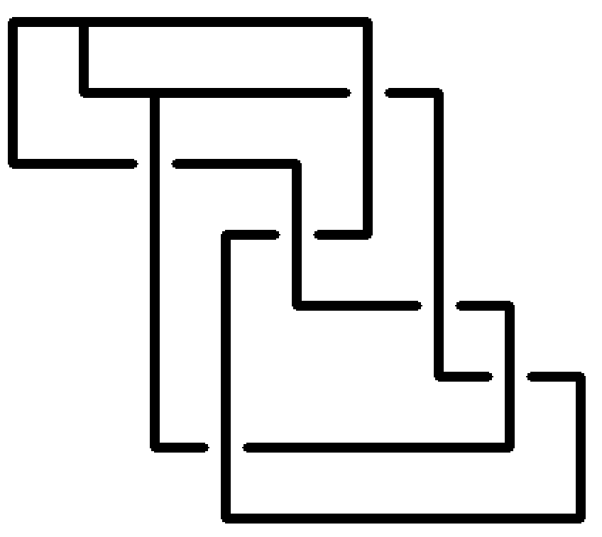
\includegraphics[width=2.5cm]{../Midterm_Poster/grid_diagram/theta_6_9.png}
    \caption{$6_9$} 
    \end{subfigure}
    \begin{subfigure}{0.075\textwidth}
    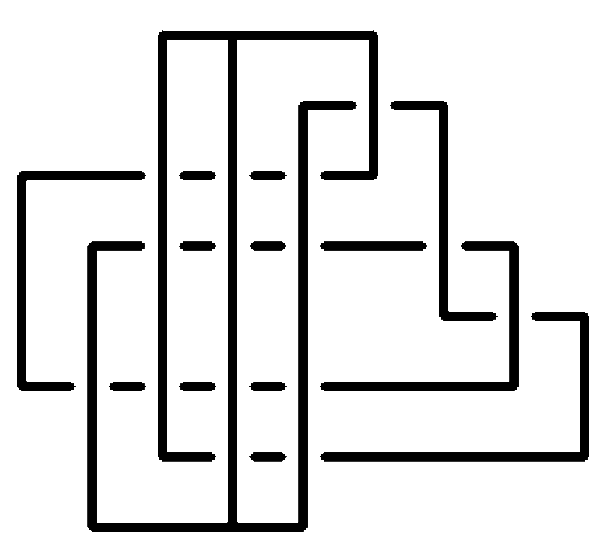
\includegraphics[width=2.5cm]{../Midterm_Poster/grid_diagram/theta_6_10.png}
    \caption{$6_{10}$} 
    \end{subfigure}
    \begin{subfigure}{0.075\textwidth}
    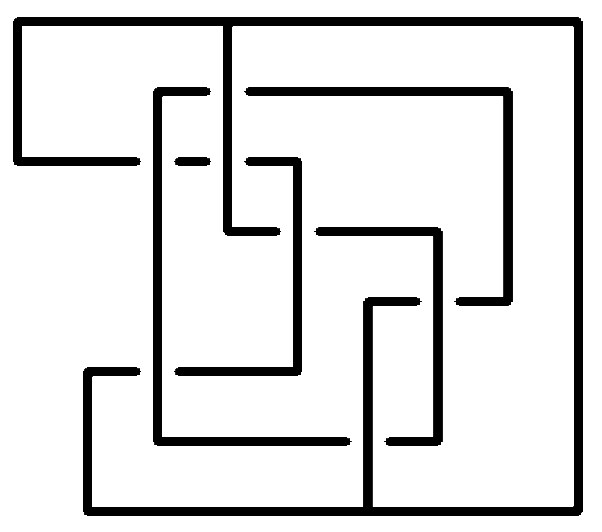
\includegraphics[width=2.5cm]{../Midterm_Poster/grid_diagram/theta_6_11.png}
    \caption{$6_{11}$} 
    \end{subfigure}
    \begin{subfigure}{0.075\textwidth}
    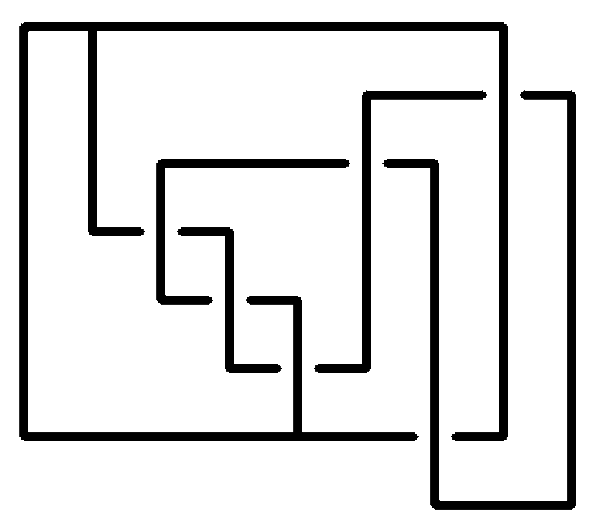
\includegraphics[width=2.5cm]{../Midterm_Poster/grid_diagram/theta_6_12.png}
    \caption{$6_{12}$} 
    \end{subfigure}
    \begin{subfigure}{0.075\textwidth}
    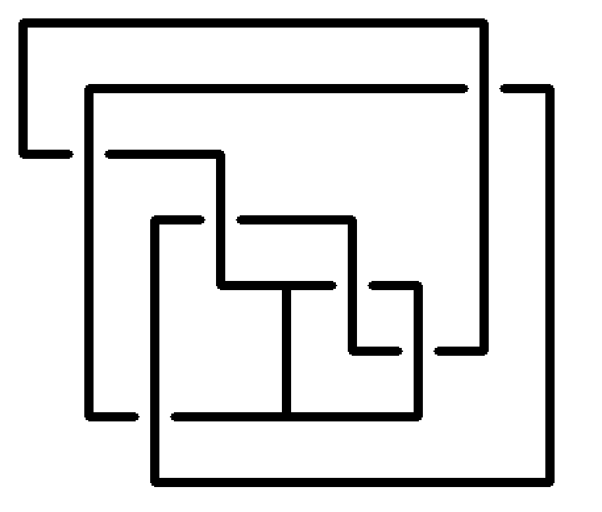
\includegraphics[width=2.5cm]{../Midterm_Poster/grid_diagram/theta_6_13.png}
    \caption{$6_{13}$} 
    \end{subfigure}
    \begin{subfigure}{0.075\textwidth}
    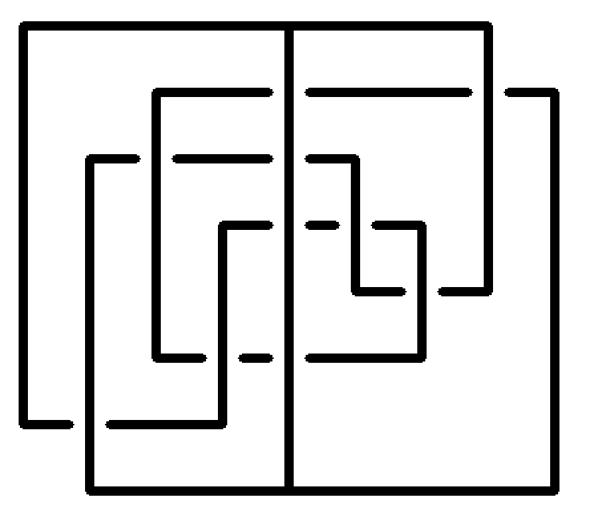
\includegraphics[width=2.5cm]{../Midterm_Poster/grid_diagram/theta_6_14.png}
    \caption{$6_{14}$} 
    \end{subfigure}
    \begin{subfigure}{0.075\textwidth}
    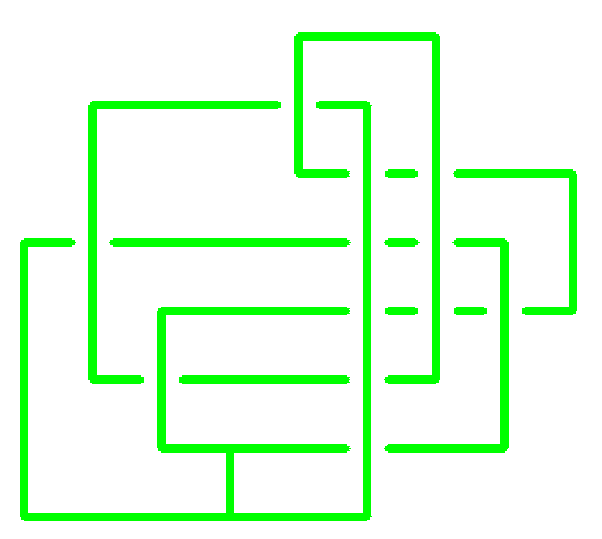
\includegraphics[width=2.5cm]{../Midterm_Poster/grid_diagram/theta_6_15.png}
    \caption{$6_{15}$} 
    \end{subfigure}
    \begin{subfigure}{0.075\textwidth}
    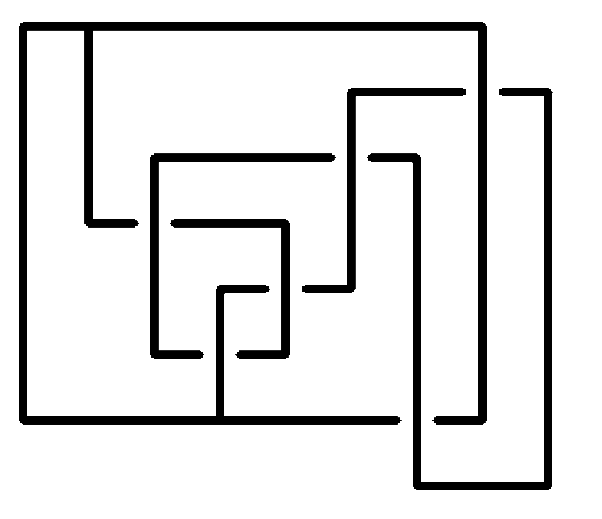
\includegraphics[width=2.5cm]{../Midterm_Poster/grid_diagram/theta_6_16.png}
    \caption{$6_{16}$} 
    \end{subfigure}
    \begin{subfigure}{0.075\textwidth}
    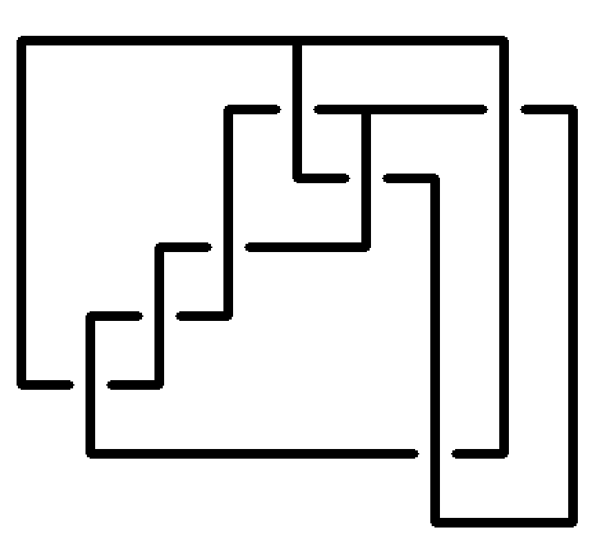
\includegraphics[width=2.5cm]{../Midterm_Poster/grid_diagram/theta_7_1.png}
    \caption{$7_{1}$} 
    \end{subfigure}
    \begin{subfigure}{0.075\textwidth}
    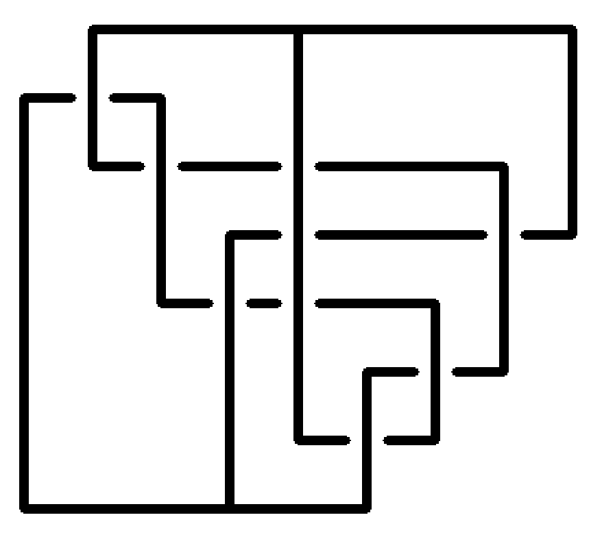
\includegraphics[width=2.5cm]{../Midterm_Poster/grid_diagram/theta_7_2.png}
    \caption{$7_{2}$} 
    \end{subfigure}
    \begin{subfigure}{0.075\textwidth}
    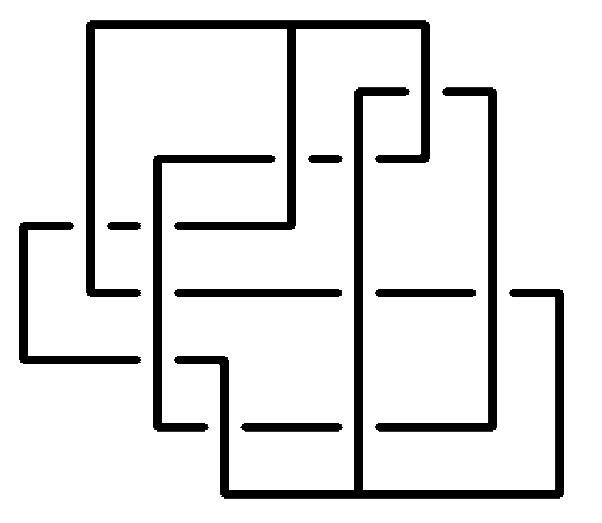
\includegraphics[width=2.5cm]{../Midterm_Poster/grid_diagram/theta_7_3.png}
    \caption{$7_{3}$} 
    \end{subfigure}
    \begin{subfigure}{0.075\textwidth}
    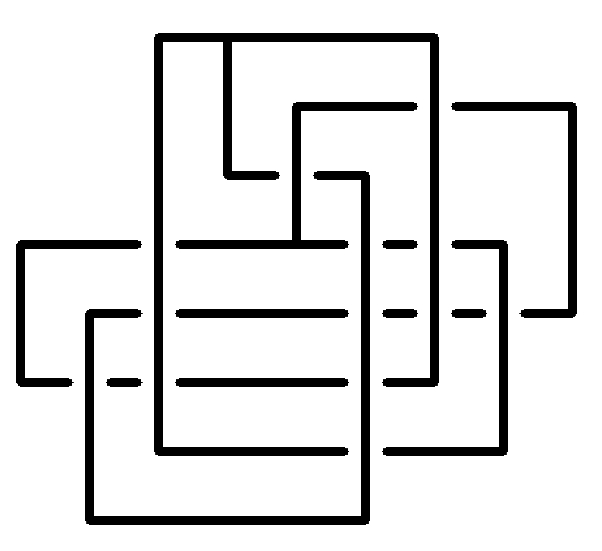
\includegraphics[width=2.5cm]{../Midterm_Poster/grid_diagram/theta_7_4.png}
    \caption{$7_{4}$} 
    \end{subfigure}
    \begin{subfigure}{0.075\textwidth}
    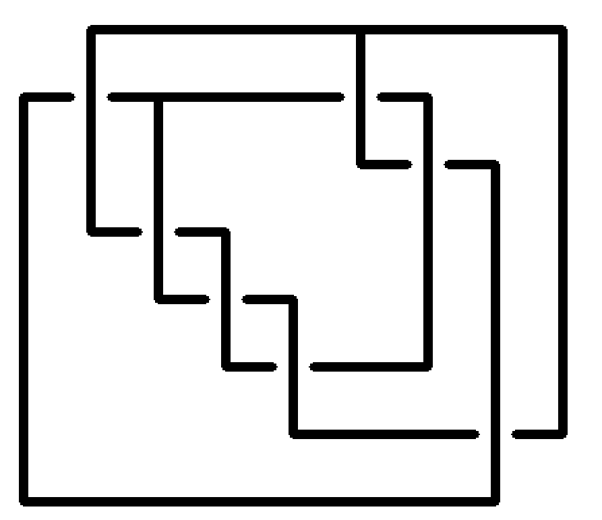
\includegraphics[width=2.5cm]{../Midterm_Poster/grid_diagram/theta_7_5.png}
    \caption{$7_{5}$} 
    \end{subfigure}
    \begin{subfigure}{0.075\textwidth}
    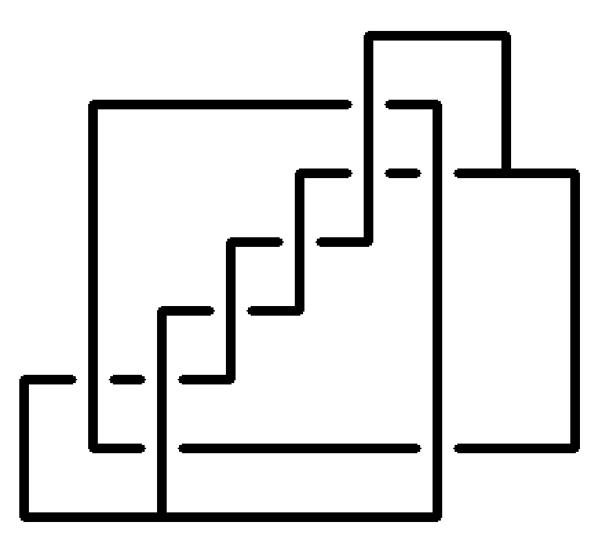
\includegraphics[width=2.5cm]{../Midterm_Poster/grid_diagram/theta_7_6.png}
    \caption{$7_{6}$} 
    \end{subfigure}
    \begin{subfigure}{0.075\textwidth}
    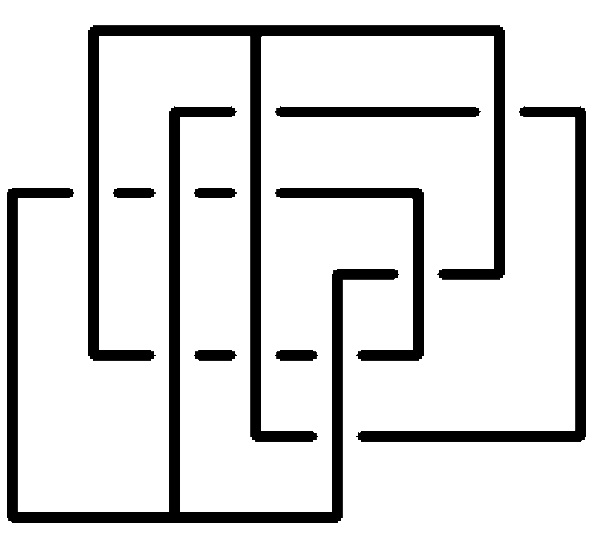
\includegraphics[width=2.5cm]{../Midterm_Poster/grid_diagram/theta_7_7.png}
    \caption{$7_{7}$} 
    \end{subfigure}
    \begin{subfigure}{0.075\textwidth}
    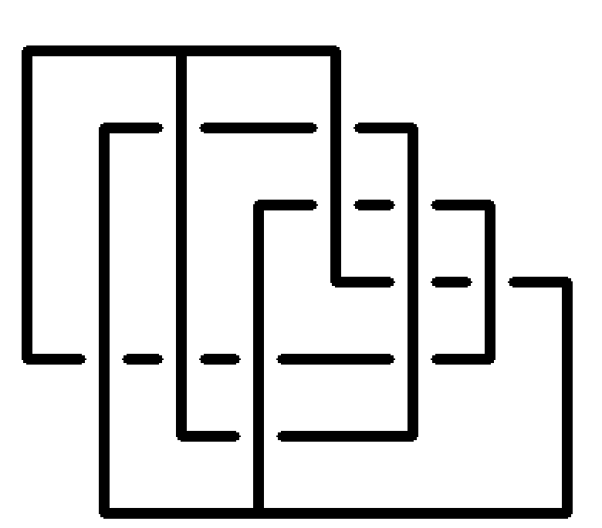
\includegraphics[width=2.5cm]{../Midterm_Poster/grid_diagram/theta_7_8.png}
    \caption{$7_{8}$} 
    \end{subfigure}
    \begin{subfigure}{0.075\textwidth}
    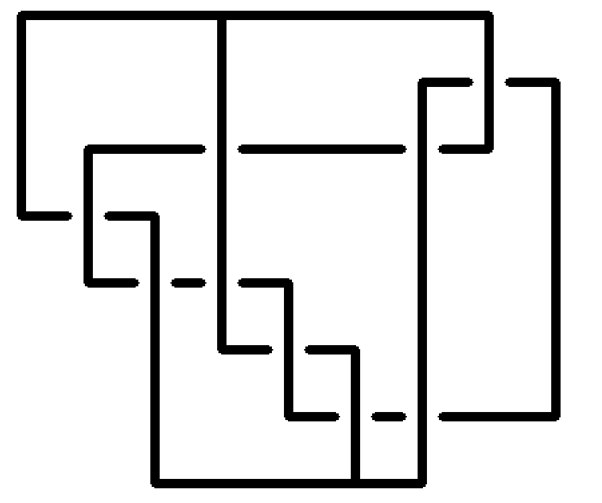
\includegraphics[width=2.5cm]{../Midterm_Poster/grid_diagram/theta_7_9.png}
    \caption{$7_{9}$} 
    \end{subfigure}
    \begin{subfigure}{0.075\textwidth}
    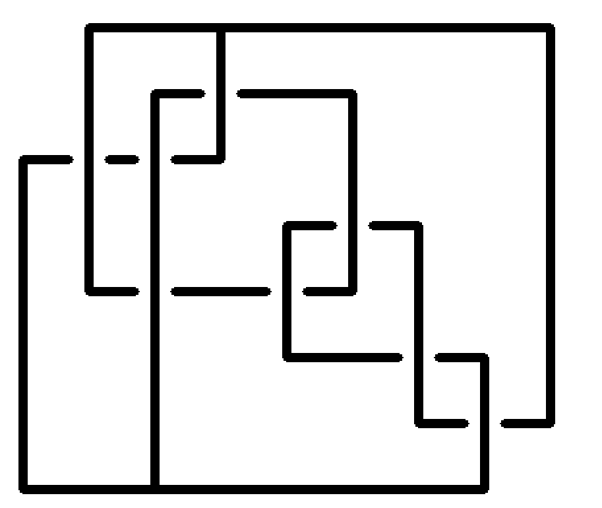
\includegraphics[width=2.5cm]{../Midterm_Poster/grid_diagram/theta_7_10.png}
    \caption{$7_{10}$} 
    \end{subfigure}
    \begin{subfigure}{0.075\textwidth}
    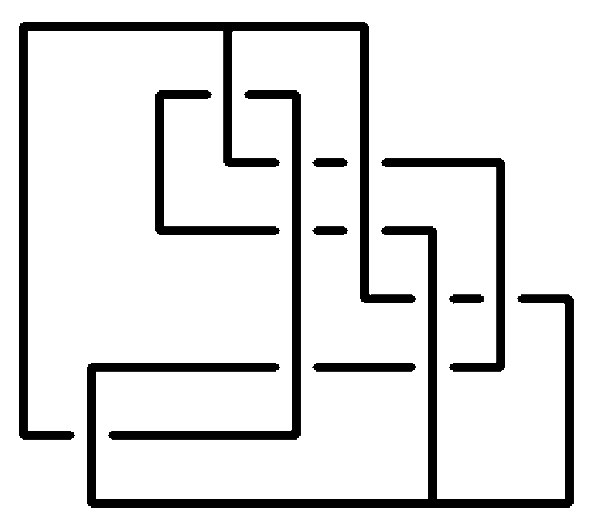
\includegraphics[width=2.5cm]{../Midterm_Poster/grid_diagram/theta_7_11.png}
    \caption{$7_{11}$} 
    \end{subfigure}
    \begin{subfigure}{0.075\textwidth}
    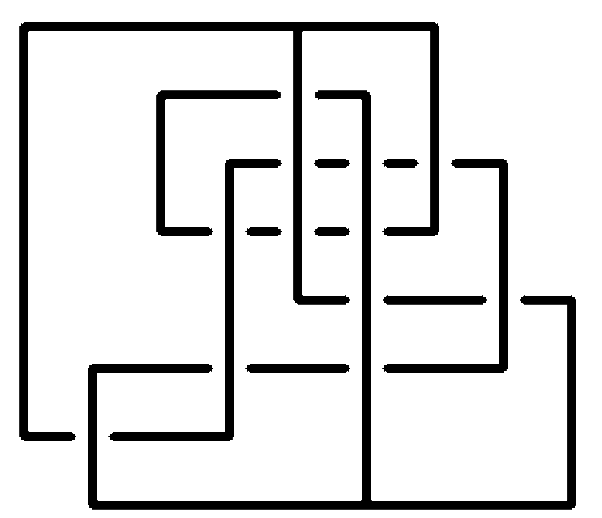
\includegraphics[width=2.5cm]{../Midterm_Poster/grid_diagram/theta_7_12.png}
    \caption{$7_{12}$} 
    \end{subfigure}
    \begin{subfigure}{0.075\textwidth}
    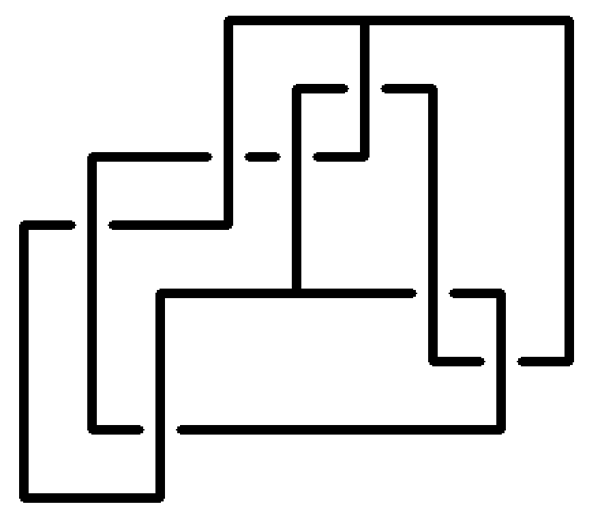
\includegraphics[width=2.5cm]{../Midterm_Poster/grid_diagram/theta_7_13.png}
    \caption{$7_{13}$} 
    \end{subfigure}
    \begin{subfigure}{0.075\textwidth}
    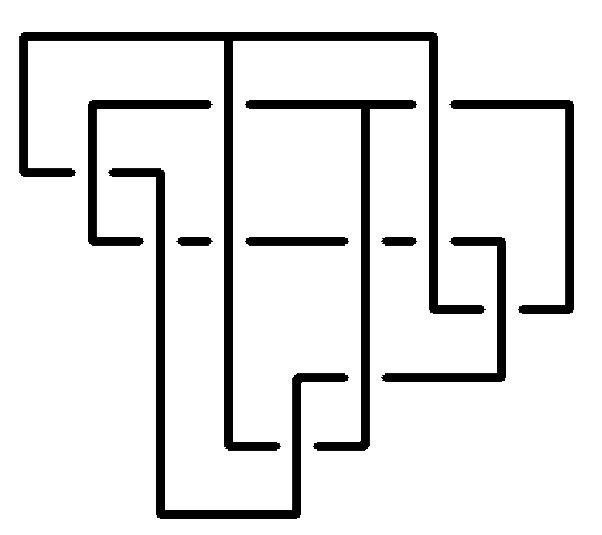
\includegraphics[width=2.5cm]{../Midterm_Poster/grid_diagram/theta_7_14.png}
    \caption{$7_{14}$} 
    \end{subfigure}
    \begin{subfigure}{0.075\textwidth}
    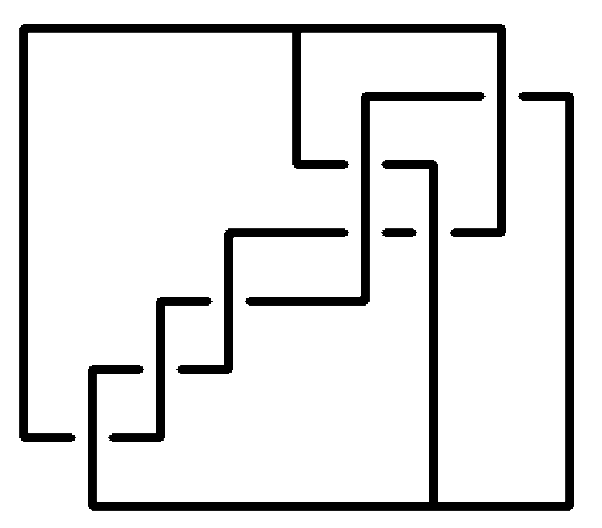
\includegraphics[width=2.5cm]{../Midterm_Poster/grid_diagram/theta_7_15.png}
    \caption{$7_{15}$} 
    \end{subfigure}
    \begin{subfigure}{0.075\textwidth}
    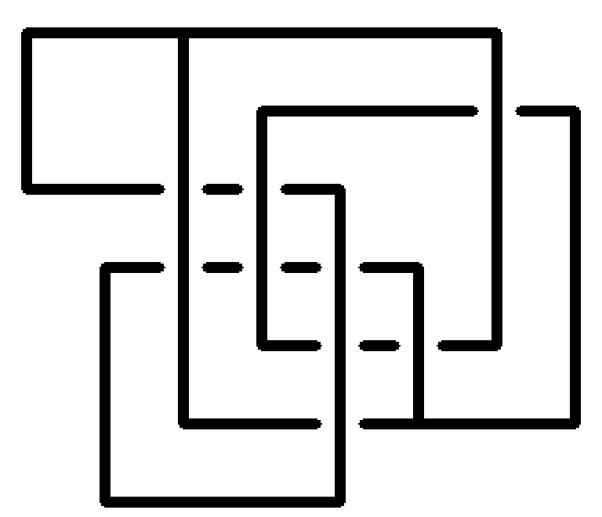
\includegraphics[width=2.5cm]{../Midterm_Poster/grid_diagram/theta_7_16.png}
    \caption{$7_{16}$} 
    \end{subfigure}
    \begin{subfigure}{0.075\textwidth}
    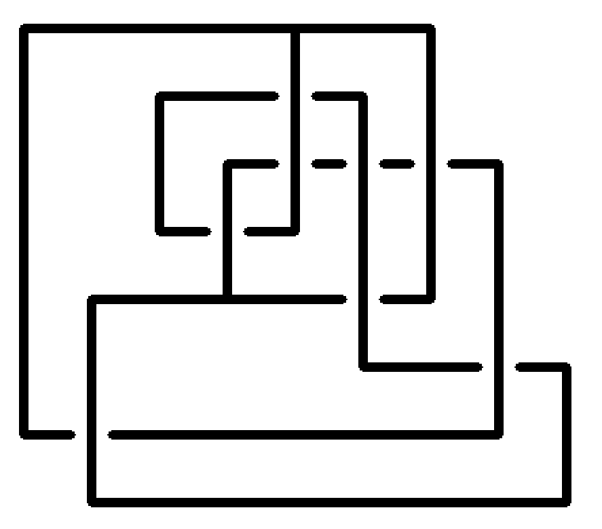
\includegraphics[width=2.5cm]{../Midterm_Poster/grid_diagram/theta_7_17.png}
    \caption{$7_{17}$} 
    \end{subfigure}
    \begin{subfigure}{0.075\textwidth}
    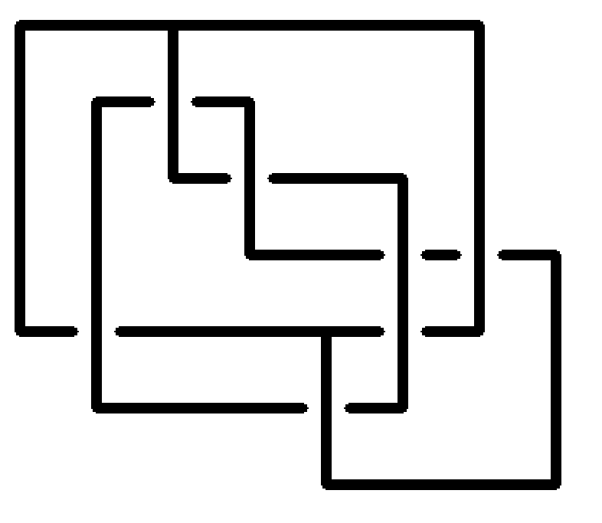
\includegraphics[width=2.5cm]{../Midterm_Poster/grid_diagram/theta_7_18.png}
    \caption{$7_{18}$} 
    \end{subfigure}
    \begin{subfigure}{0.075\textwidth}
    \includegraphics[width=2.5cm]{../Midterm_Poster/grid_diagram/theta_7_19.png}
    \caption{$7_{19}$} 
    \end{subfigure}
    \begin{subfigure}{0.075\textwidth}
    \includegraphics[width=2.5cm]{../Midterm_Poster/grid_diagram/theta_7_20.png}
    \caption{$7_{20}$} 
    \end{subfigure}
    \begin{subfigure}{0.075\textwidth}
    \includegraphics[width=2.5cm]{../Midterm_Poster/grid_diagram/theta_7_21.png}
    \caption{$7_{21}$} 
    \end{subfigure}
    \begin{subfigure}{0.075\textwidth}
    \includegraphics[width=2.5cm]{../Midterm_Poster/grid_diagram/theta_7_22.png}
    \caption{$7_{22}$} 
    \end{subfigure}
    \begin{subfigure}{0.075\textwidth}
    \includegraphics[width=2.5cm]{../Midterm_Poster/grid_diagram/theta_7_23.png}
    \caption{$7_{23}$} 
    \end{subfigure}
    \begin{subfigure}{0.075\textwidth}
    \includegraphics[width=2.5cm]{../Midterm_Poster/grid_diagram/theta_7_24.png}
    \caption{$7_{24}$} 
    \end{subfigure}
    \begin{subfigure}{0.075\textwidth}
    \includegraphics[width=2.5cm]{../Midterm_Poster/grid_diagram/theta_7_25.png}
    \caption{$7_{25}$} 
    \end{subfigure}
    \begin{subfigure}{0.075\textwidth}
    \includegraphics[width=2.5cm]{../Midterm_Poster/grid_diagram/theta_7_26.png}
    \caption{$7_{26}$} 
    \end{subfigure}
    \begin{subfigure}{0.075\textwidth}
    \includegraphics[width=2.5cm]{../Midterm_Poster/grid_diagram/theta_7_27.png}
    \caption{$7_{27}$} 
    \end{subfigure}
    \begin{subfigure}{0.075\textwidth}
    \includegraphics[width=2.5cm]{../Midterm_Poster/grid_diagram/theta_7_28.png}
    \caption{$7_{28}$} 
    \end{subfigure}
    \begin{subfigure}{0.075\textwidth}
    \includegraphics[width=2.5cm]{../Midterm_Poster/grid_diagram/theta_7_29.png}
    \caption{$7_{29}$} 
    \end{subfigure}
    \begin{subfigure}{0.075\textwidth}
    \includegraphics[width=2.5cm]{../Midterm_Poster/grid_diagram/theta_7_30.png}
    \caption{$7_{30}$}
    \end{subfigure}
    \begin{subfigure}{0.075\textwidth}
    \includegraphics[width=2.5cm]{../Midterm_Poster/grid_diagram/theta_7_31.png}
    \caption{$7_{31}$} 
    \end{subfigure}
    \begin{subfigure}{0.075\textwidth}
    \includegraphics[width=2.5cm]{../Midterm_Poster/grid_diagram/theta_7_32.png}
    \caption{$7_{32}$} 
    \end{subfigure}
    \begin{subfigure}{0.075\textwidth}
    \includegraphics[width=2.5cm]{../Midterm_Poster/grid_diagram/theta_7_33.png}
    \caption{$7_{33}$} 
    \end{subfigure}
    \begin{subfigure}{0.075\textwidth}
    \includegraphics[width=2.5cm]{../Midterm_Poster/grid_diagram/theta_7_34.png}
    \caption{$7_{34}$} 
    \end{subfigure}
    \begin{subfigure}{0.075\textwidth}
    \includegraphics[width=2.5cm]{../Midterm_Poster/grid_diagram/theta_7_35.png}
    \caption{$7_{35}$} 
    \end{subfigure}
    \begin{subfigure}{0.075\textwidth}
    \includegraphics[width=2.5cm]{../Midterm_Poster/grid_diagram/theta_7_36.png}
    \caption{$7_{36}$} 
    \end{subfigure}
    \begin{subfigure}{0.075\textwidth}
    \includegraphics[width=2.5cm]{../Midterm_Poster/grid_diagram/theta_7_37.png}
    \caption{$7_{37}$} 
    \end{subfigure}
    \begin{subfigure}{0.075\textwidth}
    \includegraphics[width=2.5cm]{../Midterm_Poster/grid_diagram/theta_7_38.png}
    \caption{$7_{38}$} 
    \end{subfigure}
    \begin{subfigure}{0.075\textwidth}
    \includegraphics[width=2.5cm]{../Midterm_Poster/grid_diagram/theta_7_39.png}
    \caption{$7_{39}$} 
    \end{subfigure}
    \begin{subfigure}{0.075\textwidth}
    \includegraphics[width=2.5cm]{../Midterm_Poster/grid_diagram/theta_7_40.png}
    \caption{$7_{40}$} 
    \end{subfigure}
    \begin{subfigure}{0.075\textwidth}
    \includegraphics[width=2.5cm]{../Midterm_Poster/grid_diagram/theta_7_41.png}
    \caption{$7_{41}$} 
    \end{subfigure}
    \begin{subfigure}{0.075\textwidth}
    \includegraphics[width=2.5cm]{../Midterm_Poster/grid_diagram/theta_7_42.png}
    \caption{$7_{42}$} 
    \end{subfigure}
    \begin{subfigure}{0.075\textwidth}
    \includegraphics[width=2.5cm]{../Midterm_Poster/grid_diagram/theta_7_43.png}
    \caption{$7_{43}$} 
    \end{subfigure}
    \begin{subfigure}{0.075\textwidth}
    \includegraphics[width=2.5cm]{../Midterm_Poster/grid_diagram/theta_7_44.png}
    \caption{$7_{44}$} 
    \end{subfigure}
    \begin{subfigure}{0.075\textwidth}
    \includegraphics[width=2.5cm]{../Midterm_Poster/grid_diagram/theta_7_45.png}
    \caption{$7_{45}$} 
    \end{subfigure}
    \begin{subfigure}{0.075\textwidth}
    \includegraphics[width=2.5cm]{../Midterm_Poster/grid_diagram/theta_7_46.png}
    \caption{$7_{46}$} 
    \end{subfigure}
    \begin{subfigure}{0.075\textwidth}
    \includegraphics[width=2.5cm]{../Midterm_Poster/grid_diagram/theta_7_47.png}
    \caption{$7_{47}$} 
    \end{subfigure}
    \begin{subfigure}{0.075\textwidth}
    \includegraphics[width=2.5cm]{../Midterm_Poster/grid_diagram/theta_7_48.png}
    \caption{$7_{48}$} 
    \end{subfigure}
    \begin{subfigure}{0.075\textwidth}
    \includegraphics[width=2.5cm]{../Midterm_Poster/grid_diagram/theta_7_49.png}
    \caption{$7_{49}$} 
    \end{subfigure}
    \begin{subfigure}{0.075\textwidth}
    \includegraphics[width=2.5cm]{../Midterm_Poster/grid_diagram/theta_7_50.png}
    \caption{$7_{50}$} 
    \end{subfigure}
    \begin{subfigure}{0.075\textwidth}
    \includegraphics[width=2.5cm]{../Midterm_Poster/grid_diagram/theta_7_51.png}
    \caption{$7_{51}$} 
    \end{subfigure}
    \begin{subfigure}{0.075\textwidth}
    \includegraphics[width=2.5cm]{../Midterm_Poster/grid_diagram/theta_7_52.png}
    \caption{$7_{52}$} 
    \end{subfigure}
    \begin{subfigure}{0.075\textwidth}
    \includegraphics[width=2.5cm]{../Midterm_Poster/grid_diagram/theta_7_53.png}
    \caption{$7_{53}$} 
    \end{subfigure}
    \begin{subfigure}{0.075\textwidth}
    \includegraphics[width=2.5cm]{../Midterm_Poster/grid_diagram/theta_7_54.png}
    \caption{$7_{54}$} 
    \end{subfigure}
    \begin{subfigure}{0.075\textwidth}
    \includegraphics[width=2.5cm]{../Midterm_Poster/grid_diagram/theta_7_55.png}
    \caption{$7_{55}$} 
    \end{subfigure}
    \begin{subfigure}{0.075\textwidth}
    \includegraphics[width=2.5cm]{../Midterm_Poster/grid_diagram/theta_7_56.png}
    \caption{$7_{56}$} 
    \end{subfigure}
    \begin{subfigure}{0.075\textwidth}
    \includegraphics[width=2.5cm]{../Midterm_Poster/grid_diagram/theta_7_57.png}
    \caption{$7_{57}$} 
    \end{subfigure}
    \begin{subfigure}{0.075\textwidth}
    \includegraphics[width=2.5cm]{../Midterm_Poster/grid_diagram/theta_7_58.png}
    \caption{$7_{58}$} 
    \end{subfigure}
    \begin{subfigure}{0.075\textwidth}
    \includegraphics[width=2.5cm]{../Midterm_Poster/grid_diagram/theta_7_59.png}
    \caption{$7_{59}$} 
    \end{subfigure}
    \begin{subfigure}{0.075\textwidth}
    \includegraphics[width=2.5cm]{../Midterm_Poster/grid_diagram/theta_7_60.png}
    \caption{$7_{60}$} 
    \end{subfigure}
    \begin{subfigure}{0.075\textwidth}
    \includegraphics[width=2.5cm]{../Midterm_Poster/grid_diagram/theta_7_61.png}
    \caption{$7_{61}$} 
    \end{subfigure}
    \begin{subfigure}{0.075\textwidth}
    \includegraphics[width=2.5cm]{../Midterm_Poster/grid_diagram/theta_7_62.png}
    \caption{$7_{62}$} 
    \end{subfigure}
    \begin{subfigure}{0.075\textwidth}
    \includegraphics[width=2.5cm]{../Midterm_Poster/grid_diagram/theta_7_63.png}
    \caption{$7_{63}$} 
    \end{subfigure}
    \begin{subfigure}{0.075\textwidth}
    \includegraphics[width=2.5cm]{../Midterm_Poster/grid_diagram/theta_7_64.png}
    \caption{$7_{64}$} 
    \end{subfigure}
    \begin{subfigure}{0.075\textwidth}
    \includegraphics[width=2.5cm]{../Midterm_Poster/grid_diagram/theta_7_65.png}
    \caption{$7_{65}$} 
    \end{subfigure}
  \end{figure}


  \end{alertblock}
\end{column}
\begin{column}{0.3\textwidth}
  \begin{alertblock}{Handcuff Graphs}
  \begin{figure}
    \begin{subfigure}{0.15\textwidth}
    \includegraphics[width=2.5cm]{../Midterm_Poster/grid_diagram/handcuff_2_1.png}
    \caption{$2_{1}$} 
    \end{subfigure}
    \begin{subfigure}{0.15\textwidth}
    \includegraphics[width=2.5cm]{../Midterm_Poster/grid_diagram/handcuff_4_1.png}
    \caption{$4_{1}$} 
    \end{subfigure}
    \begin{subfigure}{0.15\textwidth}
    \includegraphics[width=2.5cm]{../Midterm_Poster/grid_diagram/handcuff_5_1.png}
    \caption{$5_{1}$} 
    \end{subfigure}
    \begin{subfigure}{0.15\textwidth}
    \includegraphics[width=2.5cm]{../Midterm_Poster/grid_diagram/handcuff_6_1.png}
    \caption{$6_{1}$} 
    \end{subfigure}
    \begin{subfigure}{0.15\textwidth}
    \includegraphics[width=2.5cm]{../Midterm_Poster/grid_diagram/handcuff_6_2.png}
    \caption{$6_{2}$} 
    \end{subfigure}
    \begin{subfigure}{0.15\textwidth}
    \includegraphics[width=2.5cm]{../Midterm_Poster/grid_diagram/handcuff_6_3.png}
    \caption{$6_{3}$} 
    \end{subfigure}
    \begin{subfigure}{0.15\textwidth}
    \includegraphics[width=2.5cm]{../Midterm_Poster/grid_diagram/handcuff_6_4.png}
    \caption{$6_{4}$} 
    \end{subfigure}
    \begin{subfigure}{0.15\textwidth}
    \includegraphics[width=2.5cm]{../Midterm_Poster/grid_diagram/handcuff_6_5.png}
    \caption{$6_{5}$} 
    \end{subfigure}
    \begin{subfigure}{0.15\textwidth}
    \includegraphics[width=2.5cm]{../Midterm_Poster/grid_diagram/handcuff_6_6.png}
    \caption{$6_{6}$} 
    \end{subfigure}
    \begin{subfigure}{0.15\textwidth}
    \includegraphics[width=2.5cm]{../Midterm_Poster/grid_diagram/handcuff_6_7.png}
    \caption{$6_{7}$} 
    \end{subfigure}
    \begin{subfigure}{0.15\textwidth}
    \includegraphics[width=2.5cm]{../Midterm_Poster/grid_diagram/handcuff_6_8.png}
    \caption{$6_{8}$} 
    \end{subfigure}
    \begin{subfigure}{0.15\textwidth}
    \includegraphics[width=2.5cm]{../Midterm_Poster/grid_diagram/handcuff_6_9.png}
    \caption{$6_{9}$} 
    \end{subfigure}
    \begin{subfigure}{0.15\textwidth}
    \includegraphics[width=2.5cm]{../Midterm_Poster/grid_diagram/handcuff_7_1.png}
    \caption{$7_{1}$} 
    \end{subfigure}
    \begin{subfigure}{0.15\textwidth}
    \includegraphics[width=2.5cm]{../Midterm_Poster/grid_diagram/handcuff_7_2.png}
    \caption{$7_{2}$} 
    \end{subfigure}
    \begin{subfigure}{0.15\textwidth}
    \includegraphics[width=2.5cm]{../Midterm_Poster/grid_diagram/handcuff_7_3.png}
    \caption{$7_{3}$} 
    \end{subfigure}
    \begin{subfigure}{0.15\textwidth}
    \includegraphics[width=2.5cm]{../Midterm_Poster/grid_diagram/handcuff_7_4.png}
    \caption{$7_{4}$} 
    \end{subfigure}
    \begin{subfigure}{0.15\textwidth}
    \includegraphics[width=2.5cm]{../Midterm_Poster/grid_diagram/handcuff_7_5.png}
    \caption{$7_{5}$} 
    \end{subfigure}
    \begin{subfigure}{0.15\textwidth}
    \includegraphics[width=2.5cm]{../Midterm_Poster/grid_diagram/handcuff_7_6.png}
    \caption{$7_{6}$} 
    \end{subfigure}
    \begin{subfigure}{0.15\textwidth}
    \includegraphics[width=2.5cm]{../Midterm_Poster/grid_diagram/handcuff_7_7.png}
    \caption{$7_{7}$} 
    \end{subfigure}
    \begin{subfigure}{0.15\textwidth}
    \includegraphics[width=2.5cm]{../Midterm_Poster/grid_diagram/handcuff_7_8.png}
    \caption{$7_{8}$} 
    \end{subfigure}
    \begin{subfigure}{0.15\textwidth}
    \includegraphics[width=2.5cm]{../Midterm_Poster/grid_diagram/handcuff_7_9.png}
    \caption{$7_{9}$} 
    \end{subfigure}
    \begin{subfigure}{0.15\textwidth}
    \includegraphics[width=2.5cm]{../Midterm_Poster/grid_diagram/handcuff_7_10.png}
    \caption{$7_{10}$} 
    \end{subfigure}
    \begin{subfigure}{0.15\textwidth}
    \includegraphics[width=2.5cm]{../Midterm_Poster/grid_diagram/handcuff_7_11.png}
    \caption{$7_{11}$} 
    \end{subfigure}
    \begin{subfigure}{0.15\textwidth}
    \includegraphics[width=2.5cm]{../Midterm_Poster/grid_diagram/handcuff_7_12.png}
    \caption{$7_{12}$} 
    \end{subfigure}
    \begin{subfigure}{0.15\textwidth}
    \includegraphics[width=2.5cm]{../Midterm_Poster/grid_diagram/handcuff_7_13.png}
    \caption{$7_{13}$} 
    \end{subfigure}
    \begin{subfigure}{0.15\textwidth}
    \includegraphics[width=2.5cm]{../Midterm_Poster/grid_diagram/handcuff_7_14.png}
    \caption{$7_{14}$} 
    \end{subfigure}
    \begin{subfigure}{0.15\textwidth}
    \includegraphics[width=2.5cm]{../Midterm_Poster/grid_diagram/handcuff_7_15.png}
    \caption{$7_{15}$} 
    \end{subfigure}
    \begin{subfigure}{0.15\textwidth}
    \includegraphics[width=2.5cm]{../Midterm_Poster/grid_diagram/handcuff_7_16.png}
    \caption{$7_{16}$} 
    \end{subfigure}
    \begin{subfigure}{0.15\textwidth}
    \includegraphics[width=2.5cm]{../Midterm_Poster/grid_diagram/handcuff_7_17.png}
    \caption{$7_{17}$} 
    \end{subfigure}
    \begin{subfigure}{0.15\textwidth}
    \includegraphics[width=2.5cm]{../Midterm_Poster/grid_diagram/handcuff_7_18.png}
    \caption{$7_{18}$} 
    \end{subfigure}
    \begin{subfigure}{0.15\textwidth}
    \includegraphics[width=2.5cm]{../Midterm_Poster/grid_diagram/handcuff_7_19.png}
    \caption{$7_{19}$} 
    \end{subfigure}
    \begin{subfigure}{0.15\textwidth}
    \includegraphics[width=2.5cm]{../Midterm_Poster/grid_diagram/handcuff_7_20.png}
    \caption{$7_{20}$} 
    \end{subfigure}
    \begin{subfigure}{0.15\textwidth}
    \includegraphics[width=2.5cm]{../Midterm_Poster/grid_diagram/handcuff_7_21.png}
    \caption{$7_{21}$} 
    \end{subfigure}
    \begin{subfigure}{0.15\textwidth}
    \includegraphics[width=2.5cm]{../Midterm_Poster/grid_diagram/handcuff_7_22.png}
    \caption{$7_{22}$} 
    \end{subfigure}
    \begin{subfigure}{0.15\textwidth}
    \includegraphics[width=2.5cm]{../Midterm_Poster/grid_diagram/handcuff_7_23.png}
    \caption{$7_{23}$} 
    \end{subfigure}
    \begin{subfigure}{0.15\textwidth}
    \includegraphics[width=2.5cm]{../Midterm_Poster/grid_diagram/handcuff_7_24.png}
    \caption{$7_{24}$} 
    \end{subfigure}
    \begin{subfigure}{0.15\textwidth}
    \includegraphics[width=2.5cm]{../Midterm_Poster/grid_diagram/handcuff_7_25.png}
    \caption{$7_{25}$} 
    \end{subfigure}
    \begin{subfigure}{0.15\textwidth}
    \includegraphics[width=2.5cm]{../Midterm_Poster/grid_diagram/handcuff_7_26.png}
    \caption{$7_{26}$} 
    \end{subfigure}
    \begin{subfigure}{0.15\textwidth}
    \includegraphics[width=2.5cm]{../Midterm_Poster/grid_diagram/handcuff_7_27.png}
    \caption{$7_{27}$} 
    \end{subfigure}
    \begin{subfigure}{0.15\textwidth}
    \includegraphics[width=2.5cm]{../Midterm_Poster/grid_diagram/handcuff_7_28.png}
    \caption{$7_{28}$} 
    \end{subfigure}
    \begin{subfigure}{0.15\textwidth}
    \includegraphics[width=2.5cm]{../Midterm_Poster/grid_diagram/handcuff_7_29.png}
    \caption{$7_{29}$} 
    \end{subfigure}
    \begin{subfigure}{0.15\textwidth}
    \includegraphics[width=2.5cm]{../Midterm_Poster/grid_diagram/handcuff_7_30.png}
    \caption{$7_{30}$} 
    \end{subfigure}
    \begin{subfigure}{0.15\textwidth}
    \includegraphics[width=2.5cm]{../Midterm_Poster/grid_diagram/handcuff_7_31.png}
    \caption{$7_{31}$} 
    \end{subfigure}
    \begin{subfigure}{0.15\textwidth}
    \includegraphics[width=2.5cm]{../Midterm_Poster/grid_diagram/handcuff_7_32.png}
    \caption{$7_{32}$} 
    \end{subfigure}
    \begin{subfigure}{0.15\textwidth}
    \includegraphics[width=2.5cm]{../Midterm_Poster/grid_diagram/handcuff_7_33.png}
    \caption{$7_{33}$} 
    \end{subfigure}
    \begin{subfigure}{0.15\textwidth}
    \includegraphics[width=2.5cm]{../Midterm_Poster/grid_diagram/handcuff_7_34.png}
    \caption{$7_{34}$} 
    \end{subfigure}
    \begin{subfigure}{0.15\textwidth}
    \includegraphics[width=2.5cm]{../Midterm_Poster/grid_diagram/handcuff_7_35.png}
    \caption{$7_{35}$} 
    \end{subfigure}
    \begin{subfigure}{0.15\textwidth}
    \includegraphics[width=2.5cm]{../Midterm_Poster/grid_diagram/handcuff_7_36.png}
    \caption{$7_{36}$} 
    \end{subfigure}
  \end{figure}
  \end{alertblock}
  \end{column}
  \end{columns}
  \end{alertblock}

\begin{columns}[t]
  \column{0.33\textwidth}
  \begin{block}{Stacked Tangle Representation}

  \begin{itemize}
    \item \textbf{stacked tangle} : a configuration of stacked disks with arcs and caps
    \item \textbf{arcs} : segments properly embedded in each disk, with endpoints on the boundary
    \item \textbf{caps} : segments from the arc in one disk to the arc in another disk
    \item \textbf{simple closure}: the planar projection of the stacked tangle without any nested caps
  \end{itemize}
  % Then a simple closure of a stacked tangle without any nested caps is
  % corresponding to an arc presentation.

  \begin{figure}
      \centering
      \includegraphics[width=0.8\textwidth]{../Midterm_Poster/figure/stacked_tangle.png}
      \caption{Stacked tangle and simple closure of handcuff graph $2_1$}
  \end{figure}

  \end{block}
  \column{0.33\textwidth}
  \begin{block}{Bounds of Arc Index}

    $\mathbf{Definition.}$ For a graph $G$ and its edge set $E$, let
    \[ h(G)(x, y) = \sum_{F \subset E} (-x)^{-|F|} x^{\mu(G-F)} y^{\beta(G-F)}. \]
    \ ($\mu(G)$ is the number of connected components of $G$, and $\beta(G)$ is the first Betti number of $G$.) \\
    \ Then, the \textbf{Yamada polynomial} of a graph $G$, $R(G)$ is defined by
    \[ R(G)(x) = h(G)(-1, -x-2-x^{-1}). \]

    \vspace{1em}

    $\mathbf{Theorem}$ For a spatial graph $G$, $(-x)^n R(G)$ is an ambient isotopy invariant for some integer $n$.

    \vspace{1em}
    
    $\mathbf{Theorem.}$ Let $S_T$ be a simple closure of stacked tangle of a theta-curve or handcuff graph, and let $n$ be the number of crossings in $S_T$. Then,
     \[ \mathrm{spr}(R(S_T)) \leq 2n+2 \]
    where $R(S_T)$ is the Yamada polynomial of $S_T$, and $\mathrm{spr}(f)$ denotes the difference between the maximal and minimal degrees of $f$. \\

    \vspace{1em}

    $\mathbf{Corollary.}$  Let $G$ be a theta-curve or handcuff graph. Then, the arc index of $G$ is bounded by
      \[ \alpha(G) \geq \frac{5 + \sqrt{4 \mathrm{spr}(R(G)) - 15}}{2}. \]
  \end{block}
  \column{0.33\textwidth}
  \begin{block}{Refernces}
    \begin{enumerate}
      \item Yoonsang Lee. (year). \textit{A Study on Arc Index of Theta-Curves}. Korea Science Academy of KAIST
      \item H. Moriuchi. (2009). \textit{A table of 0-curves and handcuff graphs with up to seven crossings}. Advanced Studies in Pure Mathematics 55, 2009 Noncommutativity and Singularities
pp. 281-290
      \item MINJUNG LEE & SUNGJONG NO & AND SEUNGSANG OH. (2017). \textit{ARC INDEX OF SPATIAL GRAPHS}. arXiv:1711.08116v1 [math.GT] 22 Nov 2017
    \end{enumerate}
  \end{block}
\end{columns}



% \end{columns}
\end{frame}

\end{document}